\documentclass{standalone}

\usepackage{circuitikz}

\begin{document}

% INT_AY20_MP3_L27_Fig02_Area_boundary_direction.png

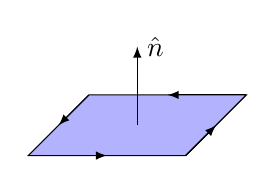
\begin{tikzpicture}[> = latex]

	% Surface
	
	\draw [fill = blue!30] (0, 0, 0) -- (0, 0, 2) -- (2, 0, 2) -- (2, 0, 0) -- (0, 0, 0);
	
	% Various arrows
	
	\begin{scope}[->]
	
		% Normal vector
	
		\draw  (1, 0, 1) -- (1, 1, 1) node [right] {${\hat n}$};
	
		% Boundary orientation
		
		\draw (0, 0, 0) -- (0, 0, 1);
		\draw (0, 0, 2) -- (1, 0, 2);
		\draw (2, 0, 2) -- (2, 0, 1);
		\draw (2, 0, 0) -- (1, 0, 0);
	
	\end{scope}

\end{tikzpicture}

\end{document}